
\chapter{Background}
In this chapter, we discuss the overall experiment of which the 408 nm 5 GHz detuned laser system is a part. We will give a detailed summary of the preparation the atoms undergo before they are exposed to our laser system. We will also attempt to sensibly contextualize the ion interferometer vis-\`a-vis other physics experiments. 

\section{Ion Interferometer Basic Overview}
The ion interferometer uses a Mach-Zehnder configuration, which refers to the fact that it relies on splitting and recombining the interfering beam of atoms. See Fig.\ \ref{mach-zehnder-fig}. 


\begin{figure}
\centerline{
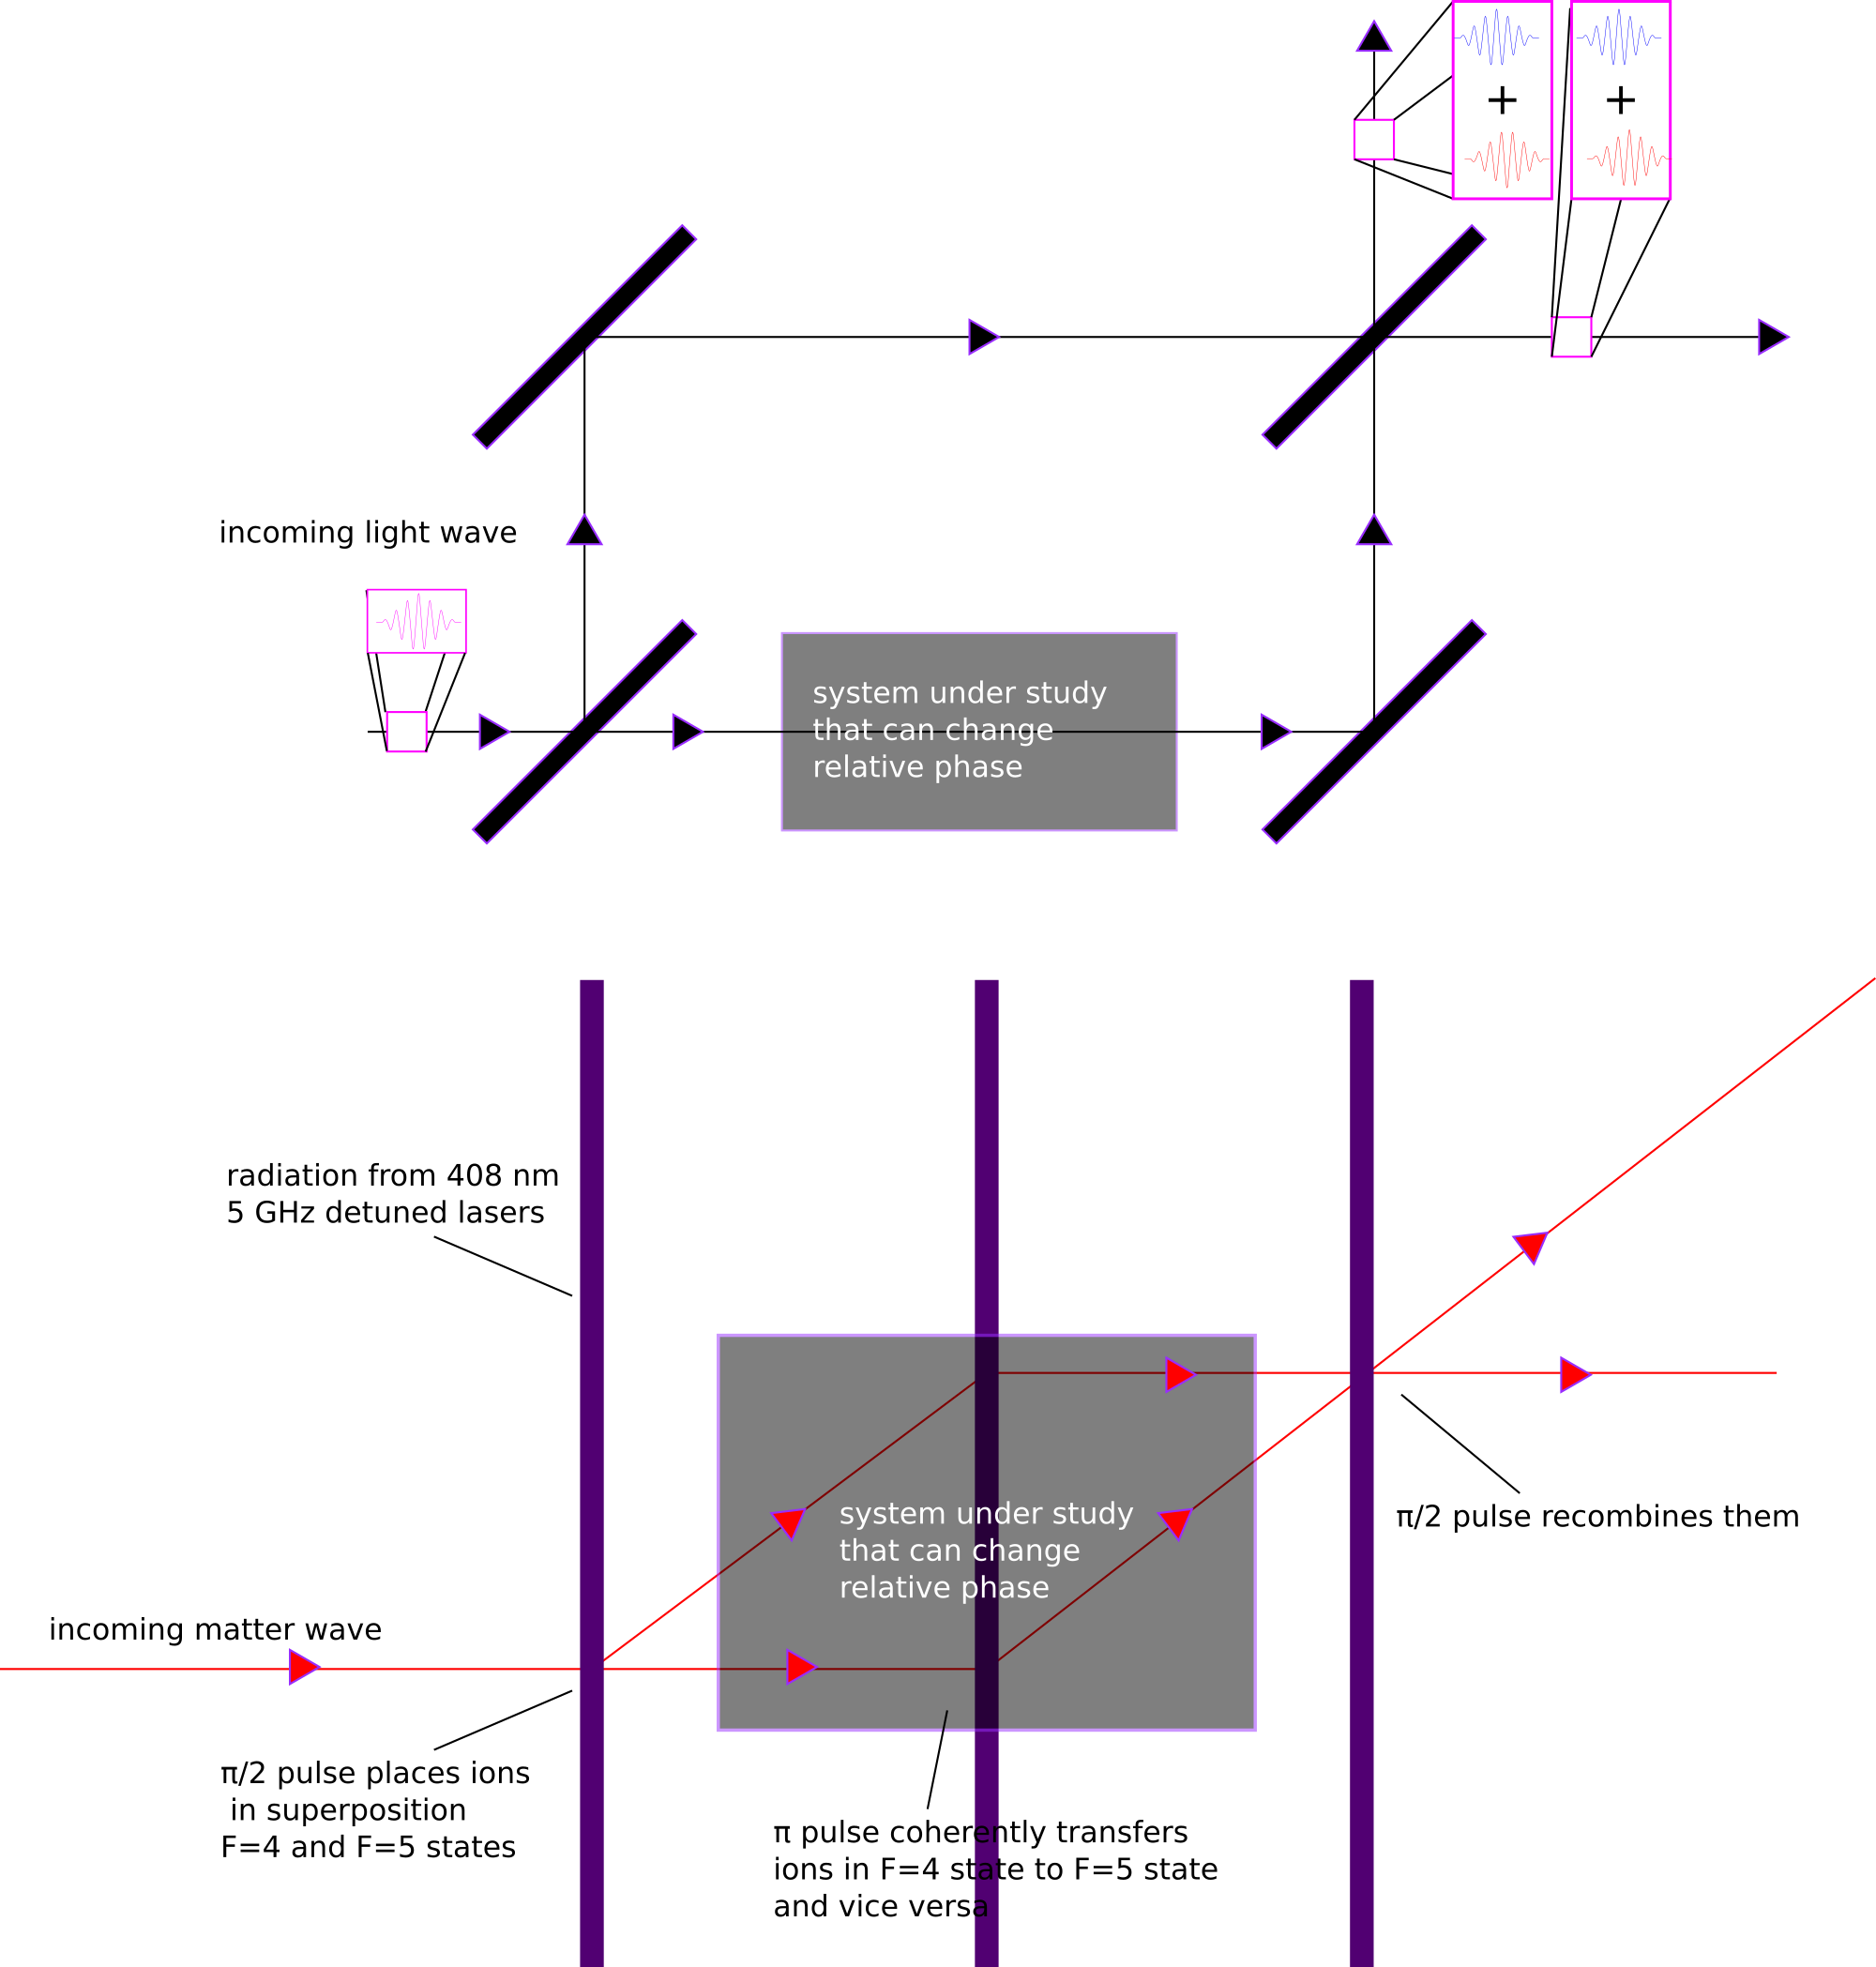
\includegraphics[width=0.95\textwidth]{mach-zehnder}}
\caption[Optical and Matterwave Mach Zehnder interferometers]{\label{mach-zehnder-fig}A traditional realization of an optical Mach Zehnder interferometer (top) juxtaposed with a sparse diagram of the ion interferometer (bottom). The ion interferometer is designed to achieve interference of matter waves and uses continuous wave lasers as its beam splitters. Notice that both involve splitting and recombining the beam. }
\end{figure}


As with any interferometer, the essential feature is that there is travelling wave that is split and sent along two paths. The output of the interferometer gives information about the relative phase shift acquired along each of the arms of the interferometer. 

The central feature of any interferometer is the splitting and recombining of waves in such a way that the relative phase difference between the two paths may be indirectly observed. In our interferometer, we plan to achieve interference of the atomic wave function of our $^{87}$Sr$^+$ ions. 
In order to accomplish ion interferometry, we must first acquire a suitable source of $^{87}$Sr$+$ ions. 

Thus, there are three basic steps associated with the operation of the interferometer. 
\begin{itemize}
\item Generation of a low velocity beam of cold Strontium atoms   
\item Ionization of Strontium Atoms
\item Atom interferometry
\end{itemize} 

The basic outline of the apparatus is illustrated in Figure~\ref{fig:IonInterferometer}.

\begin{figure}
\centerline{
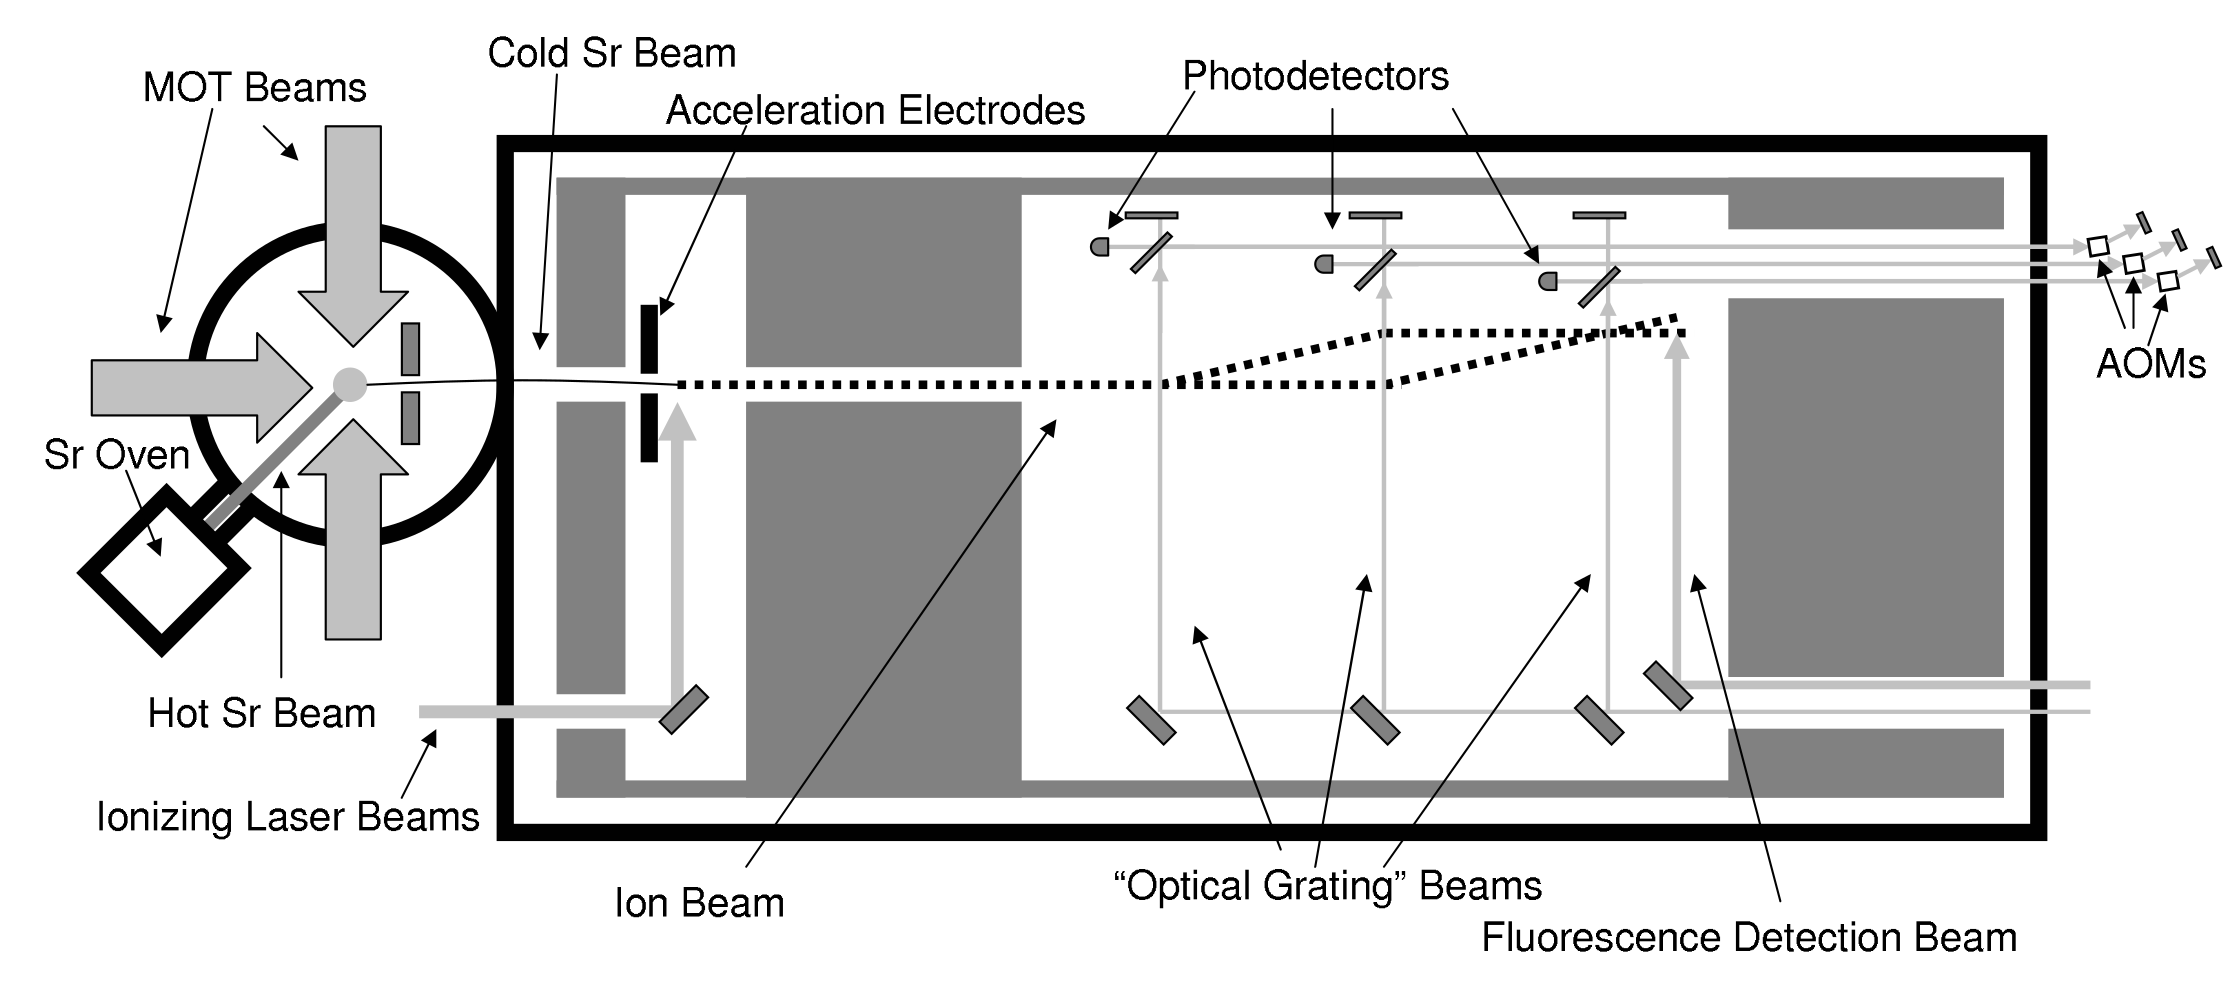
\includegraphics[totalheight=0.3\textheight]{interferometer_diagram}
}
\caption[Ion Interferometer]{\label{fig:IonInterferometer}
The entire Strontium interferometer. } 
\end{figure}

\section{Trapping of Neutral Strontium and Low Velocity Intense Source (LVIS)}

First, we must obtain a slow-moving beam of ionized $^{87}$Sr$+$. This is accomplished in two steps. 

We trap the $^{87}$Sr in a magneto-optical trap (MOT) using the standard techniques as outlined by Erickson\cite{cjeDiss}. 
The 5s$^2$ $^1$S$_0$ to 5s5p $^1$P$_1$ transition is used to cool and trap the atoms. 
The trap consists of 6 red-detuned laser beams originating from the 460.8 nm laser system described in Ref.\,\cite{cjeDiss}. These point from each of six orthogonal directions towards the center of the MOT. The dominant cooling effect in the MOT is Doppler cooling. 
The trap also relies on the magnetic field produced by a pair of permanent rare-earth magnets. This magnetic field causes the atoms to experience a Zeeman shift whose magnitude depends on their location. This process effectively confines the coldest atoms to a small region. The amount of trapped atoms is enhanced by our use of a Zeeman slower. 

Incidentally, this cooling and trapping process selects the 87u isotope of Strontium%\footnote{Further rejection of other Sr isotopes occurs because the Raman beams will not drive their transitions.}

We create an LVIS \cite{cjeDiss} following techniques developed by Cornell\cite{LVIS}. One of the mirrors in in the trap has a small hole drilled in it\footnote{This hole was drilled in-house and the details of how we avoided damage and tests that verify the integrity of its optical surface can be seen in \cite{cjeDiss}}. This allows some of the atoms to escape the trap. These atoms have a relatively narrow distribution of velocities. %\footnote{Probably cite some other reference here--whoever invented/talked about the LVIS}


The atoms that drift out of the trap are then accelerated by a sort of ``Zeeman accelerator,'' i.e. the same as the effect exploited in a Zeeman slower, but the atoms are not slowing down. The magnetic field gradients that we use for this are created by the same permanent magnets that are used to make the magnetic field gradient in the middle of the trap.

\section{Ionization of Strontium}
 
The next step is to selectively ionize the $^{87}$Sr to produce $^{87}$Sr$+$. We accomplish this using a pair of lasers tuned to resonant transitions of Sr. First, we stimulate the 5s$^2$ $^1$S$_0 \rightarrow$ 5s5p $^1$P$_1$ transition using a 461 nm laser. Conveniently, this is the same 461 nm transition used to cool the atom. The second transition is the 5s5p $^1$P$_1\rightarrow$5p$^2$ $^1$D$_2$ transition. The $^1$D$_2$ state is 57 meV above the ionization threshold \cite{NSFprop} and therefore, the Sr spontaneously autoionizes from this state. Stimulation of this transition requires a 405 nm laser. This is also a very convenient wavelength since we can drive this transition with diode lasers that are widely-produced and readily commercially available.
%\footnote{Maybe InGaN? It is the same diode laser technology used in Blu-ray players.}

After passing through the ionization lasers, the ions are accelerated by an electric field produced by two copper electrodes held at constant potential. We can control the speed of the atoms by adjusting the potential on the electrodes.%\footnote{Dallin--do I need to talk about the change in speed more? I'm kind of just talking about what happens to the atoms in sequential order, but should I justify it?}

\section{Interferometry}

After passing throught the electrodes, the ions enter the third major segment of the experiment: the interferometer. In this segment of the experiment, we use laser light as an atomic beamsplitter. At each ``atomic beamsplitter,'' we coherently manipulate the internal state of the atoms and we either split or combine the path the atoms take through this last phase of the experiment. The interference betweeen these two paths is what makes this an atom interferometer.
%the waves that are interfered are the quantum mechanical matter waves of our atoms. I borrowed the words "atomic wave function" phrase from chu and kasevich

In order to produce two distinct paths, we use stimulated Raman transitions as done by Kasevich and Chu\cite{kasevichChu1991}. We use stimulated Raman transitions. This is a two photon process: we drive the atoms from one state to another using a third state as an intermediate state. We have 3 pairs of overlapping 408 nm lasers in our apparatus and each of these pairs is tuned to induce a stimulated Raman transition between the two $^2$S$_{1/2}$ ($5s$) ground states corresponding to $F=4$ and $F=5$. The transition uses the $^2$P$_{3/2}$ ($5p$) state as an intermediate state. 

%The stimulated Raman transition process is one whereby we 

We will analyze this more completely in Chapter \ref{ChapterAboutTheAtoms}.


%trust yourself and know that you know it. and know that it doesn't have to be much better than it will be to be acceptable. 

%Is it true that at the end, we can distinguish between the F=4 and F=5 ground state of the Strontium? 
%I hope so. Those are the two states, haha. 

